\documentclass[a4paper,10pt]{article}

\usepackage{geometry}

\usepackage[utf8x]{inputenc}
\usepackage[bookmarks,colorlinks=false,pdfborder={0 0 0}]{hyperref}
\hypersetup{pdftitle={Unternehmensorientierung - Geschäftsidee: gamergeld.de}}
\usepackage{url}
\usepackage[ngerman]{babel}
\usepackage{graphicx}
\usepackage{listings}

\parindent 0pt
\parskip 10pt

\title{Unternehmensorientierung - Geschäftsidee: gamergeld.de}
\author{Erik Andresen \and Andreas Basener \and Jan Depke \and Andreas Krohn \and Benjamin Vetter}

\begin{document}

\maketitle

\section{Geschäftsidee}
\emph{Zentralisierte Zahlungsabwicklung für Browsergames/Free-to-Play Games}

Kooperation mit Gameherstellern

Gamehersteller sollten/werden mit uns kooperieren, weil
\begin{itemize}
  \item weniger Implentierungsaufwand (vor allem: neue Spiele)
  \item Verlinkung von unserer Seite - damit: Bekanntheitsgewinn
\end{itemize}

Wir bieten eine API für Gamehersteller an.
Die Wechselkurse zur jeweiligen Gamewährung werden per API übergeben.

Spieler wird z.B. beim Kauf eines Items auf gamergeld.de redirected und zahlt dort den geforderten Betrag bzw. belastet sein Konto.
Zahlung über Paypal, clickandbuy, giropay, Kreditkarte, Bankeinzug, sofortüberweisung, Moneybookers, Bitcoins, Prepaid, ..

\subsection{Risiken}
\begin{itemize}
  \item Zahlungsausfall
  \item Klar als Vermittler und nicht als Anbieter der Items kennzeichnen (Regress..)
\end{itemize}

\section{Tragfähigkeit}\label{labelTragfaehigkeit}

\subsection{Marktuntersuchung}\label{labelMarktuntersuchung}
\subsection{Wettbewerber}

\begin{itemize}
 \item Zahlungsabwicklung der Finanzinstitute
 \item Zahlungsabwicklung durch Aggregatoren
\end{itemize}

%------------------------------------------------------------------------------------

\subsubsection{Anbietertypen}

\begin{itemize}
 \item Zahlungsabwicklung der Finanzinstitute
 \item Zahlungsabwicklung durch Aggregatoren
\end{itemize}
 
%------------------------------------------------------------------------------------

\subsubsection{Realisierungstypen}

\begin{itemize}
 \item Debit-Card
 \item eigenstaendige Pseudowaehrungen
 \item Meta-Waehrungen (angestrebt)
 \item "man in the middle" fuer klassische Finanzinstitute
 \item Aggregatoren unterschiedlicher Realisierungstypen
\end{itemize}

%------------------------------------------------------------------------------------

\subsubsection{Angebotskomponenten}

\begin{itemize}
 \item Zahlungsabwicklung
 \item Transaktionspruefung
 \item Kundenpruefung
 \item Supportdienstleistung
 \item Fraud Protection
\end{itemize}

%------------------------------------------------------------------------------------

\subsubsection{Bekannte Dienstleister}

\begin{itemize}
 \item paysafecard (innerdeutsch relevant)
 \item paypal   (innerdeutsch relevant)
 \item Visa, Mastercard, Amex, Discover (innerdeutsch relevant)
 \item Giropay (innerdeutsch relevant)
 \item Bank Transfer
 \item Wallie Card
 \item Moneybookers
 \item Ultimate Game Card
 \item Ukash
 \item Visa Electron, V.me by Visa (Paypal Klon, Start 2012)
 \item Webmoney
 \item Wirecard
\end{itemize}
 

%------------------------------------------------------------------------------------

\subsubsection{Wettbewerberdaten, sofern verfuegbar und innderdeutsch relevant}

paysafecard.com Wertkarten AG   \newline \newline
Jahresumsatz 20010 i.H.v. 35 Millionen EUR 
20 Prozent Umsatz durch Sportwetten, hauptsaechlich Gluecksspiel 
Umsatz i.d. letzten Jahren regelmaessig 126 Prozent des Vorjahres  [1] \newline
\newline Zielgruppe: Onlinenutzer, die bisher noch nicht im Internet eingekauft haben, z.
Zt. ca. 20 Millionen Menschen \newline \newline
Positionierung: Erste Prepaid-Karte fuer das Bezahlen im Internet, das
Unternehmen beansprucht Themenfuehrerschaft in diesem Bereich [2] \newline
\newline
Paypal  \newline \newline
Umsatz 2010 i.H.v. 3,4 Milliarden USD [3], [4]\newline
Umsatzziel 2013 i.H.v 6-7 Milliarden USD [4]\newline 
Wachstumsmarktsegment: Mobile Zahlungen [5]\newline \newline
Visa, Mastercard, Amex, Discover \newline \newline
Umsaetze alleinstehend unbekannt, Zahlungsvariante ist Bestandteil der 
Produktpalette von Aggregatoren \newline \newline
Giropay\newline \newline
Betrieben von Postbank, Star Finanz und GAD (Volksbanken und Raiffeisenbanken)
und Fiducia IT, keine Finanzdaten verfuegbar.\newline \newline
%------------------------------------------------------------------------------------

\subsection{Markt- und Wachstumscharakteristika}

Eine Studie der VRL Finance und Welsh Assembly [A2] prognostiziert ein
Marktwachstum fuer Micropayment von jaehrlich 18 Prozent. Bis zum Jahr 2015 hat 
der innereuropaeische Mircopayment-Markt ein Volumen von 15 Milliarden EUR,
ausgehend von 6 Milliarden EUR im Jahr 2010. \newline 

Einer Studie von Harris Interactive zufolge [A3] nutzen 40 Prozent der
Internetnutzer in Deutschland Micropayment-Dienste 9,1 Mal pro Monat. Hierbei werden
Micropayment-Zahlungen als Zahlungen mit einem Wert kleiner als 10 EUR
definiert. Durchschnittlich werden pro Nutzer 19,30 EUR pro Monat ueber
Micropayment umgesetzt. \newline 

Im Jahr 2010 sind bei einem Marktvolumen von 6 Milliarden EUR somit in Europa
2,59 Millionen Micropayment-Nutzer vorhanden gewesen. [A2, A3] \newline 

Die 4 bekanntesten Browsergameanbieter, welche mittlerweile inoffiziellen
Sekundaerquellen zufolge nahezu 100 Prozent Ihres Umsatzes aus dem
Micropayment-Bereich generieren, machten im Jahr 2010 zusammen ca 30 Millionen
EUR Gewinn, siehe Abschnitt \"Browsergame-Anbieter, innerdeutsch\". Genaue
Umsatzzahlen sind hier leider nicht verfuegbar. \newline

Da der Zielmarkt der Geschaeftsidee momentan derjenige der Onlinespieleanbieter
ist, sind die Browsergameanbieter primaeres Ziel der Kundenakquise. \newline

Bei break even Umsatz von 200K EUR pro Jahr muessen 0,67 Prozent des Gewinns
dieser Browsergameanbieter als Umsatz fuer die angestrebte Unternehmung
abgeschoepft werden.  \newline 

200K EUR entsprechen bei 19,30 EUR Monatsumsatz pro User rein rechnerisch einem
Kundenstamm von unter 1000 Nutzern. \newline 

%------------------------------------------------------------------------------------

\subsection{Browsergame-Anbieter, innerdeutsch}

%------------------------------------------------------------------------------------

Gameforge AG, Karlsruhe\newline \newline
Geschaeftsbericht 2009 weist Bilanzgewinn i.H.v. 26,3 Millionen EUR aus,
Wachstum um 246 Prozent im Vergleich zum Vorjahr \newline

Blue Byte GmbH\newline \newline
Jahresbilanz (bis 31.03.2010) weist Gewinn i.H.v 208K EUR aus, Wachstum um 86
Prozent im Vergleich zum Vorjahr  (BlueByte als Micropayment-Sparte von
Ubisoft)\newline 

InnoGames GmbH, Hamburg-Harburg\newline \newline
Bilanzgewinn 2009 i.H.v. ca 3 Millionen EUR im Vergleich zu 163K EUR im Jahr
2008\newline 

Bigpoint GmbH, Hamburg\newline \newline
Bilanzgewinn 2009 i.H.v. ca 564K EUR, ist aber komplett Gewinnvortrag aus dem
Vorjahr\newline
  
\subsection{Quellen}
Quellen:
[1] \url{http://www.top1001.at/showCompany.aspx?id=11374} \newline
[2] \url{http://www.wiwo.de/unternehmen/teamprofil-paysafecard/4757148.html} \newline
[3] \url{http://files.shareholder.com/downloads/ebay/937102382x0x361552/b45137ee-aa41-4c2c-94ca-d72d5b0844be/eBay_77655_BANNERLESS.pdf} \newline 
[4] \url{http://www.heise.de/newsticker/meldung/PayPal-Umsatz-soll-sich-bis-2013-verdoppeln-1188325.html} \newline
[5] \url{http://www.bloomberg.com/news/2011-02-10/paypal-revenue-will-double-by-2013-ebay-chief-executive-john-donahoe-says.html} \newline


Allgemeine Quellen \newline \newline
[A1] \url{http://www.europeanpaymentscouncil.eu/article_preview.cfm?articles_uuid=BCFC9AFD-BDA2-FC9C-B434859EC6A9CC95}
\newline 
[A2] \url{http://digitalmedia.strategyeye.com/article/sKNP15UxWnA/2011/01/27/european_micropayments_market_to_hit_usd20bn/?nsl=molKLbkUUiv6} \newline
[A3] \url{http://www.hi-media.de/presse.html?task=get_details&news_id=141} \newline

Kunden, Finanzdaten: \newline \newline 
[K1]  https://www.ebundesanzeiger.de

% vim: fileencoding=utf8


\subsection{Technische Machbarkeit}\label{labelTechMach}

Um unsere Dienstleistung für Gamehersteller anbieten zu können verwenden wir
die individuellen APIs der spezifischen Zahlungsanbieter und bieten
unsererseits eine einheitliche API für die Gamehersteller an. Alle in diesem
Dokument genannten Zahlungsanbieter verfügen über derartige APIs, sodass diese
problemlos von uns integriert werden können. Jeder Gamehersteller kann
Zahlungstransaktionen über unsere abstrahierte API durchführen und dadurch alle
von uns verwendeten Zahlungsanbieter unterstützen. 

\subsubsection{API}
Um die Verwendung unserer API möglichst einfach zu gestalten und die API
unsererseits nicht in allen gängigen Programmiersprachen implementieren zu
müssen, bietet sich die Verwendung gängiger Protokolle an, um die API
programmiersprachen- und plattformunabhängig zu gestalten. Die API werden wir
daher REST-basiert implementieren. Durch den HTTP-Unterbau von REST kann die
API in allen gängigen Programmiersprachen problemlos und ohne zusätzlichen
Aufwand unsererseits verwendet werden. Der grobe Protokollablauf für eine
einzelne Transaktion sieht bspw. wie folgt aus:

\begin{enumerate}
  \item Der Gamehersteller erstellt eine neue Transaktion für das zuvor im Account
    erstellte Game und über einen bestimmten Betrag
  \item Die Response teilt die Transaktionskennung mit
  \item Der Gamer wird zu gamergeld.de weitergeleitet oder alternativ wird gamergeld.de
    innerhalb eines iFrames angezeigt um die Transaktion innerhalb des Spiels durchzuführen
  \item Auswahl der Zahlungsart und ggf. des Zahlungsanbieters durch den Gamer, ggf. Login
  \item Durchführung der Zahlung
  \item Benachrichtigung des Zahlungsanbieters über Erfolg/Misserfolg der Transaktion,
    bspw. über eine vom Hersteller spezifizierte URL und mit Transaktionskennung
  \item Damit ist das Protokoll abgeschlossen
\end{enumerate}

\subsubsection{Infrastruktur}
Um auch auf Wachstum über die in diesem Dokument spezifizierten Erwartungen
hinaus eingestellt zu sein und eine grundsätzlich leicht skalierbare
Architektur bei planbaren Kosten zu realisieren, bietet sich die Verwendung von
Cloud-Angeboten an. Indes muss die Verfügbarkeit der verwendenten Infrastruktur
überdurchschnittlich sein, da eine Nicht-Verfügbarkeit von gamergeld.de einen
Zahlungsausfall seitens unserer Kunden nach sich zieht.

Dabei kommen Cloud-Lösungen bzgl. der verwendeten Server-, Storage- und
Datenbank-Infrastruktur, ebenso wie Load-Balancer-Lösungen in Frage.
Storage-Lösungen sind dabei jedoch von untergeordnetem Interesse, da diese nur
bzgl. Content-Delivery (CDN) für die statischen Mediendaten, die in die Website
eingebettet sind, in Frage kommen. Große und umfangreiche Mediendaten werden
hingegen von gamergeld.de nicht vorgehalten. Beispiele für derartige
Cloud-Lösungen sind bspw. die Angebote von Amazon \cite{Amazon} und Rackspace
\cite{Rackspace}. Die Kosten eines durchschnittlichen Cloud-Servers (EC2) von
Amazon belaufen sich derzeit bei rund \$227.50 jährlich \cite{Amazon}. Amazon
gibt die Verfügbarkeit ihrer Services mit 99.95\% an \cite{Amazon}. Dennoch
müssen, zwecks Redundanz und Fehlertoleranz, mehrere Server in vorzugsweise
mehreren Rechenzentren vorgehalten werden, sodass die Kosten dafür zu Beginn
bei \$800-1500 jährlich liegen. Die exakte Anzahl zu verwendenden Servern ist
abhängig vom Traffic und Transaktionsvolumen. Unsere Architektur ist auch
kurzfristig skalierbar.

Bzgl. der Datenbanken verwenden wir keine zusätzlichen Cloud-basierten
Datenbanken wie bspw. Amazon RDS, sondern verwenden MySQL- und
MongoDB-Datenbanken, die sich auf den von uns betriebenen Servern befinden.
Das hat den zusätzlichen Vorteil, dass bspw. Kundendaten ausschließlich auf
Systemen gespeichert sind, die von uns administriert werden. Die
MySQL-Datenbanken werden für Account- und andere Kundendaten verwendet,
betreiben eine Master-Slave und/oder Master-Master Replikation und sind daher
bzgl. der Read-Anweisungen gut skalierbar. Bzgl. der Write-Anweisungen wird
jedoch nur moderate Skalierbarkeit erreicht. Häufige Änderungen an Account- und
Kundendaten sind jedoch idR. nicht zu erwarten, sodass hierbei keine Probleme
entstehen. Für die Speicherung von Transkationsdaten sind die MySQL-Systeme bei
hohen Transaktionsvolumina jedoch, ohne umfangreiche Maßnahmen, nur bedingt
geeignet. Daher vewenden wir für die Transaktionensdaten MongoDB-Datenbanken,
ebenfalls mit Master-Slave und Master-Master Replikation, da NoSQL-Datenbanken
bzgl. der Write-Anweisungen einfacher zu skalieren sind\footnote{Bspw. da
Sharding bei denormalisierten Datenbanken deutlich einfacher zu realisieren
ist.}.

\subsubsection{Sicherheit}
Insider-Angriffe seitens des Cloud-Anbieters können wir nur z.T.
berücksichtigen. Jedoch dürfen Account-, Kunden-, Kreditkarten- und
Transaktionsdaten serverseitig ausschließlich auf Systemen gespeichert werden,
die von uns administriert werden. Da wir keine zusätzlichen Cloud-basierten
Datenbanken verwenden ist dies jedoch gewährleistet.

Da gamergeld.de u.a. Kreditkartendaten entgegennimmt und speichert, gelten für
die verwendeten System besonders hohe Sicherheitsanforderungen und
Schutzkategorien. Unter anderem müssen unsere Systeme die PCI-Compliance Tests
bestehen \cite{PCI}, die für alle Unternehmen und Systeme, die
Kreditkartendaten verarbeiten, gelten. Das ist mit entsprechenden
Schutzmaßnahmen, als auch mit Kosten für die PCI-Compliance-Tests verbunden.
Die Kosten für derartige Tests müssen idR. vierteljährlich durchgeführt werden,
sind abhängig von der Anzahl verwendeter IP-Adressen als auch von den
Transaktionvolumina. Pro IP-Adresse und Quartal belaufen sich die Kosten pro
IP-Adresse daher bei ca. 220 EUR \cite{PCI:Costs}, also ca. 4000 EUR jährlich
für das beschriebene Setup.

Bzgl. der Serversicherheit werden ausserdem typische Best-Practices, wie
Policies und Patch-Zyklen, Firewalls, verschlüsselte Kommunikation (SSH, SSL),
Authentifikation, etc. verwendet.


\newpage
\subsection{Finanzierung und wirtschaftliche Machbarkeit}\label{labelWirtMach}
%Gesamtplan 3-5 Jahre

Für die Berechnung unserer Finanzierung und der wirtschaftlichen Machbarkeit werden folgende Annahmen getroffen:

Als einzelne Kostenpositionen erwarten wir folgende Posten:
\begin{itemize}
\item Fixkosten
 \begin{itemize}
\item Serverkosten
\item Personalkosten
\item Büromiete
\item Kredittilgungen
 \end{itemize}
\item variable Kosten
\begin{itemize}
\item Marketingkosten
\item Entwicklungskosten
\item Transaktionsgebühren
\item Kreditzinsen
\item Bürobedarf/Sonstiges
\end{itemize}
\end{itemize}

Die Kosten für die Server ergeben sich aus den Betrachtungen im Kapitel \ref{labelTechMach}. Die vermuteten Kosten für das Büro sind dem aktuellen Hamburger Mietspiegel entnommen. Die Personalkosten verteilen sich auf die fünf Mitglieder dieses Unternehmens. Der für die Finanzierung benötigte Kredit erzeugt mit Zinsen und Tilgungen weitere Kosten.\\
Um die Kunden gewinnen zu können entstehen uns Kosten, die unter Marketingkosten zusammengefasst werden. Diese werden im laufe der Zeit abnehmen, wenn unser Bekanntheitsgrad ansteigt.\\
Die benötigte Software zur Zahlungsabwicklung mit den Kunden wird von uns selber entwickelt. Die veranschlagten Kosten sind unter dem Punkt Entwicklungskosten berücksichtigt. Die Entwicklungskosten werden im Laufe der Zeit abnehmen und werden um Wartungskosten ergänzt.\\
Weitere Kosten sind im Punkt Bürobedarf/Sonstiges zusammengefasst und können nur grob geschätzt werden.

Wie in Kapitel \ref{labelMarktuntersuchung} beschrieben, existieren diverse Spieleanbieter am Markt, die jeweils einen hohen Jahresumsatz erzielen. \\
Wir wollen mit unsren Kunden eine langfristige Geschäftsbeziehung eingehen. Wir setzen dabei darauf, dass wir nur einige wenige Kunden benötigen. Durch diese wenigen Kunden können wir aber hohe Umsätze erzielen.

Die Strategie, die wir bei der Kundengewinnung verfolgen, ist, dass wir zu Anfang mit einem Kunden starten und dann nach und nach weitere Kunden gewinnen. 

\subsubsection*{Gewinn und Verlustrechnung}
%24 auf monatlicher Basis, danach jährlich

\begin{figure}[htbp]
	\centering
	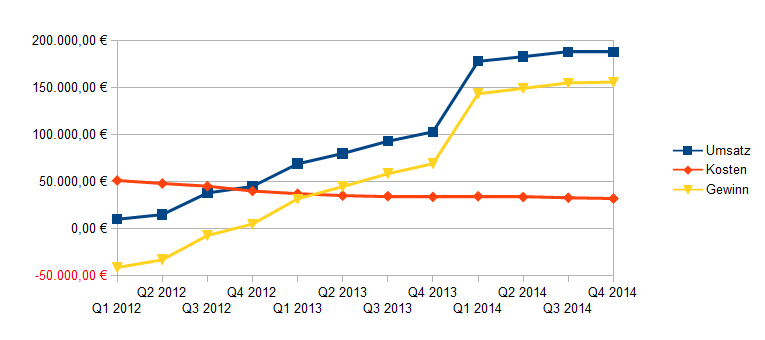
\includegraphics[width=1\textwidth]{GuV.png} 
	\caption{GuV}
	\label{picGuV}
\end{figure}

Die zu erwartenden Kosten betragen pro Quartal im Schnitt ca{.} 40.000,- Euro in den ersten 3 Jahren. Um Kostendecken arbeiten zu können müssen wir diesen Betrag über die Transaktionsgebühren wieder einholen. Wenn wir einen Anteil von 5\% an den Geldtransaktionen für uns einbehalten, dann müssen pro Quartal 800.000,- Euro bei den Kunden umgesetzt werden. 

Wie in Kapitel \ref{labelMarktuntersuchung} dargestellt, sind das sehr vorsichtige Berechnungen. Es ist davon auszugehen, dass der Umsatz bei den Kunden höher liegen wird. Dadurch können wir einerseits unsere eigenen Umsätze erhöhen und Gewinne einfahren, andererseits aber auch den prozentualen an den Kundenumsätzen verringern, was uns einen Vorteil bei Vertragsverhandlungen mit den Kunden einbringt.

\subsubsection*{Liquiditätsrechnung}
%24 auf monatlicher Basis, danach jährlich
\begin{figure}[htbp]
	\centering
	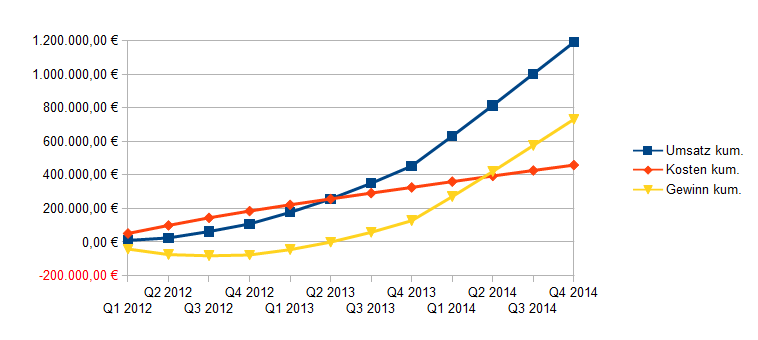
\includegraphics[width=1\textwidth]{GuVkummuliert.png}
	\caption{GuV kumuliert}
	\label{picGuVkum}
\end{figure}

Der Break-Even Punkt wird im vierten Quartal 2012 überschritten. Bis zum vorhergehenden Quartal addieren sich die Verluste auf ca{.} 82.000,- Euro (s. Abbildung \ref{picGuVkum}). Dieser Betrag wird mindestens benötigt, um die zu erwartenden Kosten zu decken.\\
Die Deckung der Kosten wird durch eine Bankfinanzierung geschehen. Dazu nehmen wir einen Kredit in Höhe von 90.000,- Euro mit einer Laufzeit von 4 Jahren und einem Zinssatz in Höhe von 5\%. Die monatlichen Tilgungsraten betragen 1.875,- Euro. Die Kosten sind in den übrigen Berechnungen bereits enthalten.


\section{Optimierung durch Analyse der Informationen}\label{labelRelDaten}
% Von Anfang an alle relevanten Daten zu sammeln und in geeigneter Form festzuhalten (Stich-
% worte: Metriken, Datawarehouse, Business Intelligence)


Zur ständigen Qualitätsverbesserung und Entwicklung des Vorsprungs gegenüber Wettbewerbern müssen unsere Dienste ständig optimiert werden.
Dazu werden wir über unsere Webseite große Mengen an Daten erheben und daraus folgende Informationen erschließen:\\
Wie oft bzw wann benutzen die Spieler unsere Seite, bzw die Spieleseite zur Zahlungsabwicklung?\\
Wann wird ein Zahlungsvorgang abgebrochen? Gibts es korrelierende Daten, die man den Browserspielen, der Zahlungsart oder einer Postleitzahl/Ort zuorden kann?\\
Kundenflüsse beobachten: Gibt es Spieler, die von uns auf andere Spiele aufmerksam werden? Welche ähnlichen Spiele kann man Zahlungswilligen Spielern noch empfehlen?\\
Kann man größere Mengen von Zahlungsausfällen zu bestimmten Regionen/Postleitzahlgebieten zuorden? Oder gibt es Browserspiele mit einer besonders hohen Quote an Zahlungsausfällen?
Wenn sich solche Browserspiele identifizieren lassen kann man diese mit höhren Gebühren belasten als Browserspiele, die höhere Umsätze erzielen bei geringerer Ausfallquote.
Bei Spielern aus Regionen mit hoher Zahlungsausfallquote kann man die Zahlungsart auf weniger Risikoreiche varianten wie Vorauskasse beschränken.\\
Erkennung rückläufiger Umsätze: Gibt es Browserspiele oder Zahlungsarten die insgesamt profitabler sind als andere? Welche Browserspiele erzielen den meisten Gewinn?
Tendenzielle Rückläufe bei den Zahlungen müssen schnell erfasst und gegebenfalls den Spielemachern mitgeteilt werden damit diese rechtzeitig neue Innovationen (und damit Gründe für Spieler,
Geld auszugeben) in ihr Spiel einbauen können.

Gesammelt werden die Daten ausschließlich über das Benutzerverhalten.
In den Daten muss genau gespeichert werden welcher Spieler wann vom welchem Spiel welchen Zahlungsvorgang bei welchem Anbieter mit welcher Summe durchführt oder wo abbricht:
Zur Auswertung der Daten werden multidimensional fähige Werkzeuge benötigt, also Werkzeuge aus dem Bereich des "`Online Analytical Processing"' um die für uns wichtigen Ergebnisse
nach z.B. Wohnort, Spiel und Zahlungsart darzustellen.\\
Eine mögliche Information kann auch sein, daß Wartungsarbeiten am besten Nachts zwischen 3 und 4 durchgeführt werden können, da dort die Wahrscheinlichkeit eines Zahlungausfalls am geringsten ist.\\
Informationen über Abbrüche beim Zahlungsvorgang und die Beziehungen welcher Spieler von welchem Portalen unsere Dienste benutzen kann man eher mit Web-Mining gewinnen.
Dabei können so möglicherweise keine Information gewonnen werden, wieso der Zahlungsvorgang abgebrochen wurde: War der User verunsichert oder hat er die Anleitung nicht verstanden?
Um diese Fragen zu beantworten sind weitere Usability-Studien erforderlich.\\
Auch Usability-Verbesserungen sind möglich, wie z.B. Zahlungsarten die je nach Spiel/User häufiger verwendet werden, können auf der Seite weiter oben angesiedelt werden.

\section{Projektplan/Geschäftsplan}\label{labelGeschaeftsplan}
Krohn
% Ergebnisse der Validierung zusammenfassen...

\bibliographystyle{plain}
\bibliography{protokoll}

\end{document}

% vim: fileencoding=utf8
